%!TEX root = ../Thesis.tex
\section{Gradient decent optimization}

A neural network have no closed form solution for optimizing the parameters $w_{i,j}$. Thus the weights must be optimized using an iterative algorithm. Gradient decent is the most common algorithm for optimizing neural networks, though many variations exists.

The basic principal is that given a loss function $\mathcal{L}$ the parameters $w_{i,j}$ can be optimized by going in the opposite direction of the gradient $\frac{\partial \mathcal{L}}{\partial w_{i,j}}$. Thus each iteration $n$ is given by:
\begin{equation}
\begin{aligned}
w_{i,j}^n = w_{i,j}^{n-1} + \Delta w_{i,j}^n, && \Delta w_{i,j}^n = - \eta_n \frac{\partial \mathcal{L}}{\partial w_{i,j}}
\end{aligned}
\end{equation}

$\eta_n$ is the \textit{stepsize} and should be so small that it doesn't skip over the wanted minima, but also not so small that weights doesn't converge within reasonable time. Typically the initial weights $w^0_{i,j}$ is given by a random distribution. The choice of stepsize and initialization are not obvious as it typically depends on the specific architecture of the network and the dataset. Furthermore different sources uses very different approaches and variations of gradient decent. For example Alex Graves \cite{alexgraves} suggests using a uniform distribution in the range $[-0.1, 0.1]$ or a normal distribution with $\sigma = 0.1$ and a constant stepsize $\eta_n = 10^{-5}$.

\subsection{Momentum}

A major problem with the naïve gradient decent algorithm, is that it tends to get stuck in a local minima because $\frac{\partial \mathcal{L}}{\partial w_{i,j}} = 0$ in such minima. To avoid this problem a \textit{momentum} can be added to the gradient decent equation:

\begin{equation}
\Delta w_{i,j}^n = - m \Delta w_{i,j}^{n-1} - \eta_n \frac{\partial \mathcal{L}}{\partial w_{i,j}}
\end{equation}

Here $m$ is the \textit{momentum} parameter. Alex Graves suggests using $m = 0.9$ \cite{alexgraves}.

\subsection{Socastic gradient decent}

For calculating the gradient some dataset is used, the naïve approach is to use the entire dataset at once. However it turns out that a better approach is to calculating the gradient using a single datapoint, then updating the parameters and repeating for all datapoints (see Algorithm \ref{algorithm:gradientdecent:SGD}). This method is called \textit{stocastic gradient decent} (SGD) or \textit{online learning}, where the naïve approach is called \textit{batch learning}.

\begin{algorithm}[h]
 \DontPrintSemicolon
 \While{stopping criteria not met}{
  Randomise training set order\;
  \For{each observation in the training set}{
   Run forward and backward pass to calculate the gradient\;
   Update weights with gradient descent algorithm\;
  }
 }
 \caption{Stocastic graident decent \cite{alexgraves}.}
 \label{algorithm:gradientdecent:SGD}
\end{algorithm}

One reason for \textit{stocastic gradient decent} being better is that it handels redundancies\todo{Why was this} in the data better. It also helps in not getting stuck in a local minima, because it is unlikely that what is a local minima for one datapoint is also a local minima for another datapoint \cite{bishop}.

\subsection{Mini-batch socastic gradient decent}

While \textit{stocastic gradient decent} is way better than \textit{batch learning} it doesn't handle outliers very well, because the gradient will be big for such observation. It also isn't very computational efficient because the vectorization libraries can't take full advantage of the CPU cache and etc..

To solve those issues \textit{Mini-batch socastic gradient decent} or \textit{mini-batch learning} is used. This is a compromise between \textit{batch learning} and \textit{online learning}, where small random batches of observations are created and the weights are then optimized like in Algorithm \ref{algorithm:gradientdecent:SGD}. This introduces a third parameter called the \textit{mini-batch-size}, which as the same suggests controls the size of the mini-batches. This also generalizes \textit{online learning} and \textit{batch learning}, because if \textit{mini-batch-size = 1} then it is \textit{online learning} and if \textit{mini-batch-size = training-size} then it is \textit{batch learning}. Generally the \textit{mini-batch-size} is just chosen by benchmarking, calculating or guessing what is the most computational efficient choose.

\begin{algorithm}[h]
 \DontPrintSemicolon
 \While{stopping criteria not met}{
  Randomise training set order\;
  Create minibatches of size \textit{mini-batch-size}\;
  \For{each minibatch in the training set}{
   Run forward and backward pass to calculate the gradient\;
   Update weights with gradient descent algorithm\;
  }
 }
 \caption{Mini-batch gradient descent.}
 \label{algorithm:gradientdecent:mini-batch}
\end{algorithm}

\subsection{RMSprop}
\todo[inline]{Introduce RMSprop.}

\subsection{Early stopping}

Optimization of the loss function $\mathcal{L}$ using just \textit{gradient decent}, is given to be non-increasing for each iteration \cite{bishop}. For this reason it is quite easy to find a minima for the training data, however this does not directly reflect the performance of the model given new data. In Figure \ref{fig:theory:gradientdecent:overfit} the loss function for the training data (green) is forever decreasing. The loss function for data not used in the training (blue) is only decreasing for the first 15 iterations, after this the performance of the model is getting worse. This is quite common and is called overfitting, an simple way to prevent this is to use \textit{early stopping}.

\textit{Early stopping} uses a third dataset, this dataset can not be used for calculating the gradients (training data) or for evaluating the model performance (test data). It is used for evaluating the loss function for each iteration and stop the optimization algorithm when the loss function haven't decreased for some iterations. \cite{the-elements-of-statistical-learning, bishop, alexgraves}

\begin{figure}[h]
	\centering
	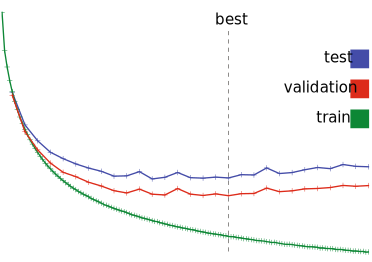
\includegraphics[scale=0.7]{theory/gradientdecent-overfit}
	\caption{Loss function for each iteration. The validation dataset indicates when to stop (the best line). However this does not excatly reflect the loss function of test dataset. Data is from \cite{alexgraves}.}
	\label{fig:theory:gradientdecent:overfit}
\end{figure}

There are other methods to prevent overfitting such as regularization \cite{the-elements-of-statistical-learning, bishop}. However only \textit{early stopping} was used in the Sutskever paper \cite{sutskever}.
